\chapter{Qulalitäts-Management}
\section{Software-Qualitätsmangement}
\subsubsection{Hauptanliegen:}
\begin{enumerate}
    \item organisatorische Ebene: schaffen eines Gerüstes aus organisatorischen Prozessen und Standards
    \item Projekt-Ebene: Anwendung spezigfischer QM-Prozesse, Kontrolle von deren Einhaltung
    \item Projekt-Ebene: Erstellung eines Qulitätsplanes, legt Ziele, Prozesse und Standards fest
\end{enumerate}

\subsubsection{Qulitätsmangement}
\begin{itemize}
    \item QM-Team muss unabhängig vom Entwicklerteam sein
    \item Kontrolle von Devlierables zur Sicherstellung der Unternehmensstandards
\end{itemize}

\subsection{Qualitätsplan}
\begin{itemize}
    \item Produktqualität, Qualitätsbewertung, Qualitätsmerkmale, Standards
    \item Bewertungsprozess
    \item Auswahl oder Neudefinition von Unternehmensstandards
    \item Aufbau:
    \begin{itemize}
        \item Produkteinführung
        \item Produktplan: Veröffentlichungsdaten, Verantwortlichkeiten, \dots
        \item Qualitätsziele
        \item Risiken und Risikomanagement
    \end{itemize}
\end{itemize}
\subsubsection{Probleme:}
\begin{enumerate}
    \item Spannung zwischen den Anforderungen von Kunde und Entwickler an die Qualität 
    \item eindeutige Formulierung von Qualitätsanforderungen schwer 
\end{enumerate}

\subsection{Software-Qualitätsattribute}
\begin{tabular}{|c|c|c|}
\hline
Sicherheit & Verständlichkeit & Protabilität \\\hline
Schutz & Testbarkeit & Benutzbarkeit \\\hline
Zuverlässigkeit & Anpassbarkeit & Wiederverwenbarkeit \\\hline
Ausfallsicherheit & Modularität & Effizienz \\\hline
Robustheit & Komplexität & Elernbarkeit \\\hline
\end{tabular}

\subsubsection{Prozess- und Produktqualität}
\begin{itemize}
    \item \textbf{\underline{Produktstandards}} definieren Charakteristiken, die alle Software-Komponenten aufweisen sollen 
    \item \textbf{\underline{Prozessstandards}} definiere, wie der Software-Prozess ausgeführt werden soll 
\end{itemize}
\begin{tabular}{|c|c|}
\hline
\textbf{Produkt-Standard} & \textbf{Prozess-Standards} \\\hline
Form des Design-Reviews & Ausführung des Desing-Reviews \\\hline
Struktur des Anforderungsdokumentes & Einreichen von neuem Code \\\hline 
Format der Methodenköpfe & Versions-Veröffentlichungsverfahren \\\hline
Programmierstil & Annahme des Projektsplanes \\\hline
Format des Projektplanes & Änderungskontrolle \\\hline
\end{tabular}
\subsection{ISO 9001 - Struktur}
\begin{itemize}
    \item Internationaler Satz von Standards $\rightarrow$ Grundlage für die Entwciklung von Qualitätsmanagement-Systemen
    \item gelten für Unternehmen, die Produkte entwerfen, entwickeln und unterhalten
    \item ISO 9001 speziell für Softwareentwicklung
    \begin{itemize}
        \item allgemeine Qualitätsprinzipien
        \item allgemine Qualitätsverfahren
        \item Auflistung von Unternehmensstandards und -verfahren
    \end{itemize}
\end{itemize}
\begin{figure}[h]
    \centering
    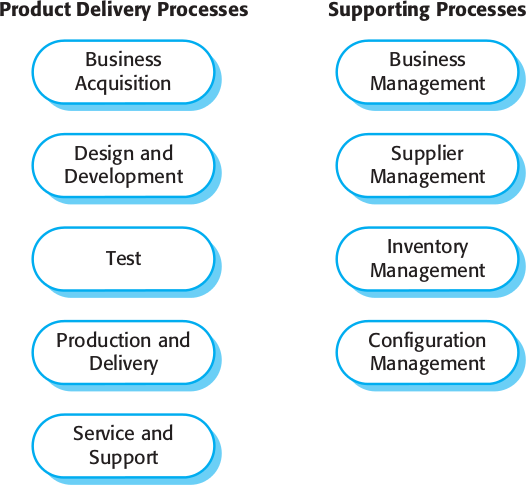
\includegraphics[width=0.5\textwidth]{mainmatter/pics/iso.png}
    \caption{ISO 900 Kern-Prozesse}
\end{figure}
\begin{itemize}
    \item ISO 9001-Zertifikation
    \begin{itemize}
        \item Qualitätsmanagement-Handbuch des Unternehmens 
        \item Externe Stelle bescheinigt die Einhaltung der ISO 9001-Standards
        \item zunehmende flexiblie Handhabung notwendig
    \end{itemize}
\end{itemize}
\begin{figure}[h]
    \centering
    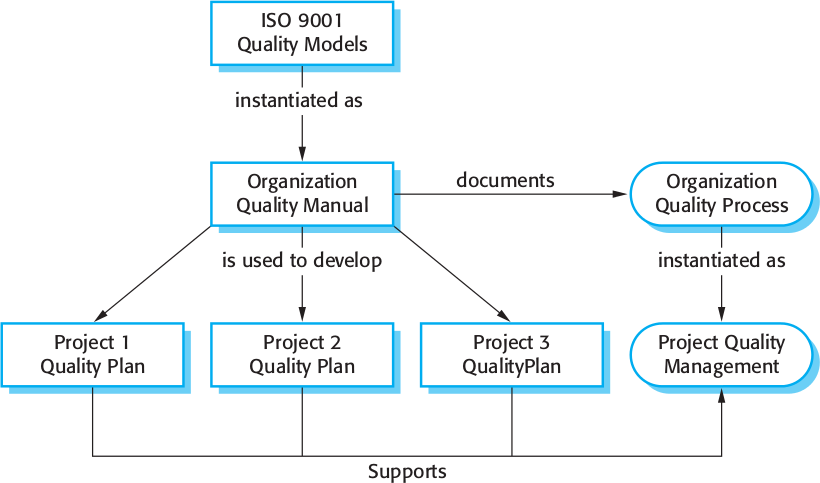
\includegraphics[width=0.75\textwidth]{mainmatter/pics/iso_9001.png}
    \caption{ISO 9001-Qualitätsmanagement}
\end{figure}


\section{Reviews and Inspections}
\begin{itemize}
    \item Gruppe kontrolliert Prozess oder System und Dokumentation $\rightarrow$ mögliche Probleme finden
    \item Akzeptanz eines Iteratinsschrittes durch die Projektleitung dokumentiert
    \item geprüft werden können: Code, Design, Spezifikationen, Testpläne, Standards, \dots
    \item \textbf{\underline{Sollten durch Checklisten gesteuert werden!}}
\end{itemize}

\subsection{Reviews agiler Methoden} 
\begin{itemize}
    \item Prüfprozess informell
    \item Extreme Programming: Pair Programming stellt kosntante Kontrolle und Überprüfung des codes durch das andere Teammitglied sicher. 
\end{itemize}

\subsection{Software measurement and metrics}
\begin{itemize}
    \item Software measurement: Entwicklung eines numerischen Wertes für Eigenschaften eines Softwareproduktes ode -prozesses
    \item Ermöglicht objektiven Vergleich zwischen Techniken und Prozessen
\end{itemize}
\subsubsection{Software metric}
\begin{itemize}
    \item jede Form von Vermessung eines Software-Systems, -prozesses oder -dokumentation
    \begin{itemize}
        \item Lines of code, Fog Index, Antahl der Arbeitstage pro Person, \dots
    \end{itemize}
    \item Software kann in Zahlen ausgedrückt werden
    \begin{itemize}
        \item Vorhersage von Produkteigenschaften, Kontrolle der Softwareprozesse
        \item Identifikation regelwiedriger Komponenten
    \end{itemize}
\end{itemize}

\subsubsection{Dynamische und statische Product Metrics}
\begin{itemize}
    \item \textbf{Dynamische Metriken:} während der Ausführung aufgenommen
    \begin{itemize}
        \item verwandt mit Qualitätseigenschaften $\rightarrow$ Effizienz, Zuverlässikgeit
        \item einfach gemessen werden können: response time (Performance-Eigenschaft), Fehlerfrequenz (Zuverlässigkeits-Eigenschaft)
    \end{itemize}
    \item \textbf{Statische Metriken:} berechnet aus Sstemdarstellungen
    \begin{itemize}
        \item indirekte Verwandschaft mit Qualitätseigenschaften
        \item Beurteilung von Komplexität, Verständlichkeit und Unterhaltbarkeit
    \end{itemize}
\end{itemize}

\section{Prozessverbesserung}
Steigerung der Produktqualität und/oder Kostenreduktion, Verkürzung der Entwicklungszeit

\subsubsection{Herangehensweisen:}
\begin{itemize}
    \item \textbf{Prozessreife-Ansatz:} Prozess- und Projektmangement-Verbesserung $\rightarrow$ \textit{good practice}
    \begin{itemize}
        \item \underline{Level der Prozessreife:} Ausmaß der Anwendung von guten technischen und Führungsmethoden
    \end{itemize}
    \item \textbf{Agiler Ansatz:} iterative Entwicklung und REduktion von Overheads im Softwareprozess 
    \begin{itemize}
        \item schnelle Auslieferung und REaktion auf Anforderungsänderungen
    \end{itemize}
\end{itemize}

\subsection{Prozessqualität}
\begin{figure}[h]
    \centering
    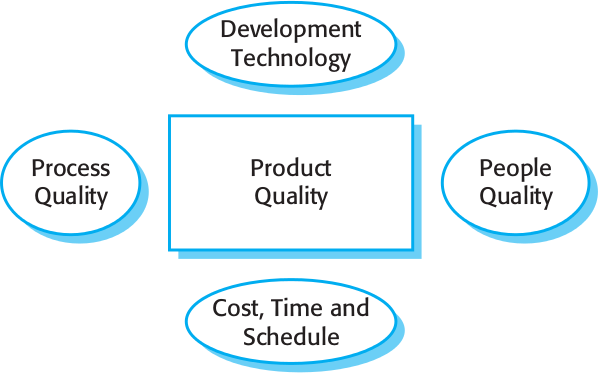
\includegraphics[width=0.5\textwidth]{mainmatter/pics/product_quality.png}
    \caption{Einflüsse auf die Softwarequalität}
\end{figure}
\begin{itemize}
    \item Großes Projekt, mittlere Fähigkeiten: Entwicklungsprozess bestimmt die Produktqualität
    \item Kleines Projekt: Fähigkeiten und Entwicklungsmethoden bedeutend 
    \item realistischer Zeitplan essentiell
\end{itemize}
\subsubsection{Beispiele für Prozess-Messgrößen:}
\begin{itemize}
    \item Dauer von Prozessaktivitäten 
    \item Benötigte Ressourcen
    \item Häufigkeit des Auftretens bestimmter Ereignisse 
\end{itemize}
\begin{figure}[h]
    \centering
    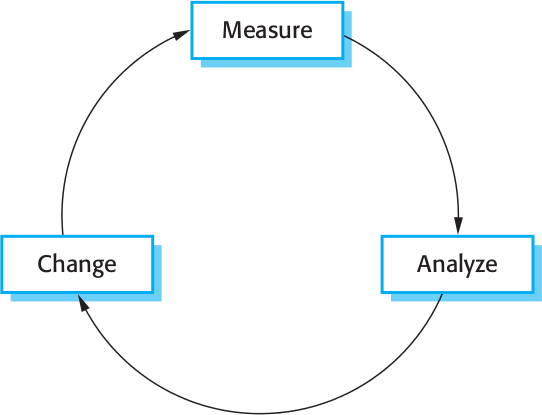
\includegraphics[width=0.40\textwidth]{mainmatter/pics/improvement_cycle.png}
    \caption{Prozess improvement cycle}
\end{figure}

\subsubsection{Prozessanalyse-Techniken:}
\begin{itemize}
    \item Veröffentlichte Prozessmodelle und -standards
    \begin{itemize}
        \item existierenden Modelle können nach Bedarf erweitert und verändert werden
    \end{itemize}
    \item Fragebögen und Interviews
    \begin{itemize}
        \item Gefahr: nicht wahrheitsgemäße Antworten
    \end{itemize}
    \item Ethnographische Analysen (Informationsgewinnung durch Beobachtung)
\end{itemize}
\begin{figure}[h]
    \centering
    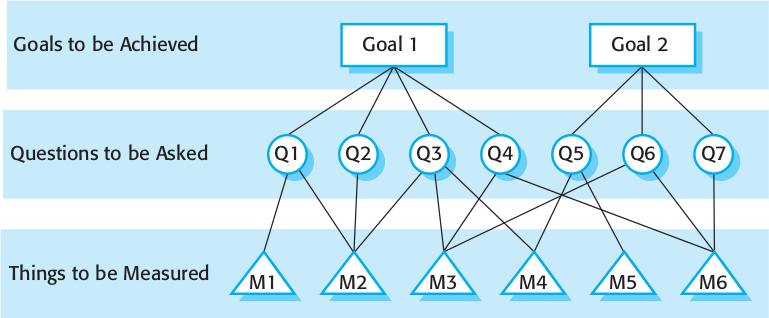
\includegraphics[width=0.75\textwidth]{mainmatter/pics/cqm_paradigm.png}
    \caption{CQM paradigm (Goals, Questions Measurements)}
\end{figure}
\begin{itemize}
    \item \underline{Modifikation existierender Prozesse}
    \item beinhaltet: 
    \begin{itemize}
        \item Einführung neuer Praktiken, Methoden, Prozesse 
        \item Änderungen der Anordnung von Prozessaktivitäten
        \item Einführung oder Entferung von Deliverables
        \item Einführung neuer Rollen und Verantwortlichkeiten 
        \item \dots
    \end{itemize}
    \item Probleme:
    \begin{itemize}
        \item Wiederstand gegen Veränderungen
        \item beständigkeit von Veränderung (Institutsionalisierung von Veränderungen sicher Beibehaltung)
    \end{itemize}
\end{itemize}
\begin{figure}[h]
    \centering
    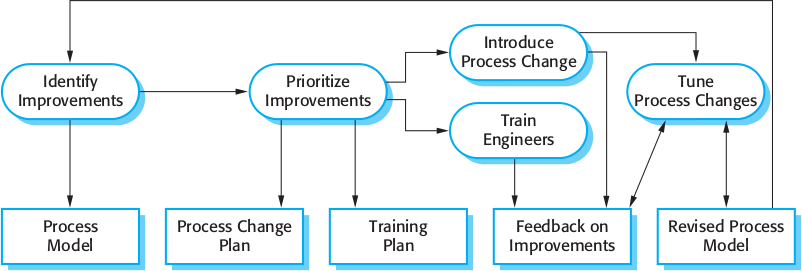
\includegraphics[width=0.75\textwidth]{mainmatter/pics/process_chainging.png}
    \caption{Prozessänderung}
\end{figure}
